\documentclass{article} % For LaTeX2e
% We will use NIPS submission format
\usepackage{nips13submit_e,times}
% for hyperlinks
\usepackage{hyperref}
\usepackage{url}
% For figures
\usepackage{graphicx} 
% math packages
\usepackage{amsmath}
\usepackage{amsfonts}
\usepackage{amsopn}
\usepackage{ifthen}
\usepackage{natbib}
\usepackage{caption}
\usepackage{subcaption}

\title{Project-I by Group Rome}

\author{
Viviana Petrescu\\
EPFL \\
\texttt{vpetresc@epfl.ch} \\
}

% The \author macro works with any number of authors. There are two commands
% used to separate the names and addresses of multiple authors: \And and \AND.
%
% Using \And between authors leaves it to \LaTeX{} to determine where to break
% the lines. Using \AND forces a linebreak at that point. So, if \LaTeX{}
% puts 3 of 4 authors names on the first line, and the last on the second
% line, try using \AND instead of \And before the third author name.

\nipsfinalcopy 

\begin{document}

\maketitle

\begin{abstract}
We present our on two tasks, classification and regression on data that is not known. We process the data, investigate baseline methods and present our results here.
For the regression task, out best model was <> and for classification was <>.
\end{abstract}

\section{Regression}
\subsection{Data Description}
The training data $Xtrain$ contains 1400 observations, each 43 dimensional. One training sample has 36 real valued features and 7 categorical features. Our task is to predict the values for unseen test data, consisting in 600 samples. We measure the accuracy of our estimation using $RMSE$. 

\subsection{Data visualization and cleaning}
Initially, our data was not centered, as seen in $Fig.$ \ref{fig:dist_regression}.
We changed the categorical features into dummy variables, leading to a new vector of size 56. $Xtrain$ was then normalized to have 0 mean and standard deviation 1. We applied the same operations to the test data $Xtest$ on which we will report the results.

 We plotted the correlation of every feature with respect to the output $ytrain$ and the scatter plots did not look random. We concluded the features explain the output, but we could not tell if one of them is insignificant.

The predicted values were real values in $[1000,7000]$ and seemed to be grouped into two blobs. We believed initially the smaller blob represented outliers, but since it contained almost $10\%$ of the data we decided not to ignore it.

After looking at every feature individually, we noticed that feature 36 offers a clear separation of the two blobs (see $Fig.$ \ref{fig:feature36}). We therefore chose to fit two models, one in which feature 36 has values $>1.4$ (after normalization) and one in which it is smaller, corresponding to smaller predicted values. 


\begin{figure}[ht]
  \begin{subfigure}[b]{0.45\textwidth}
   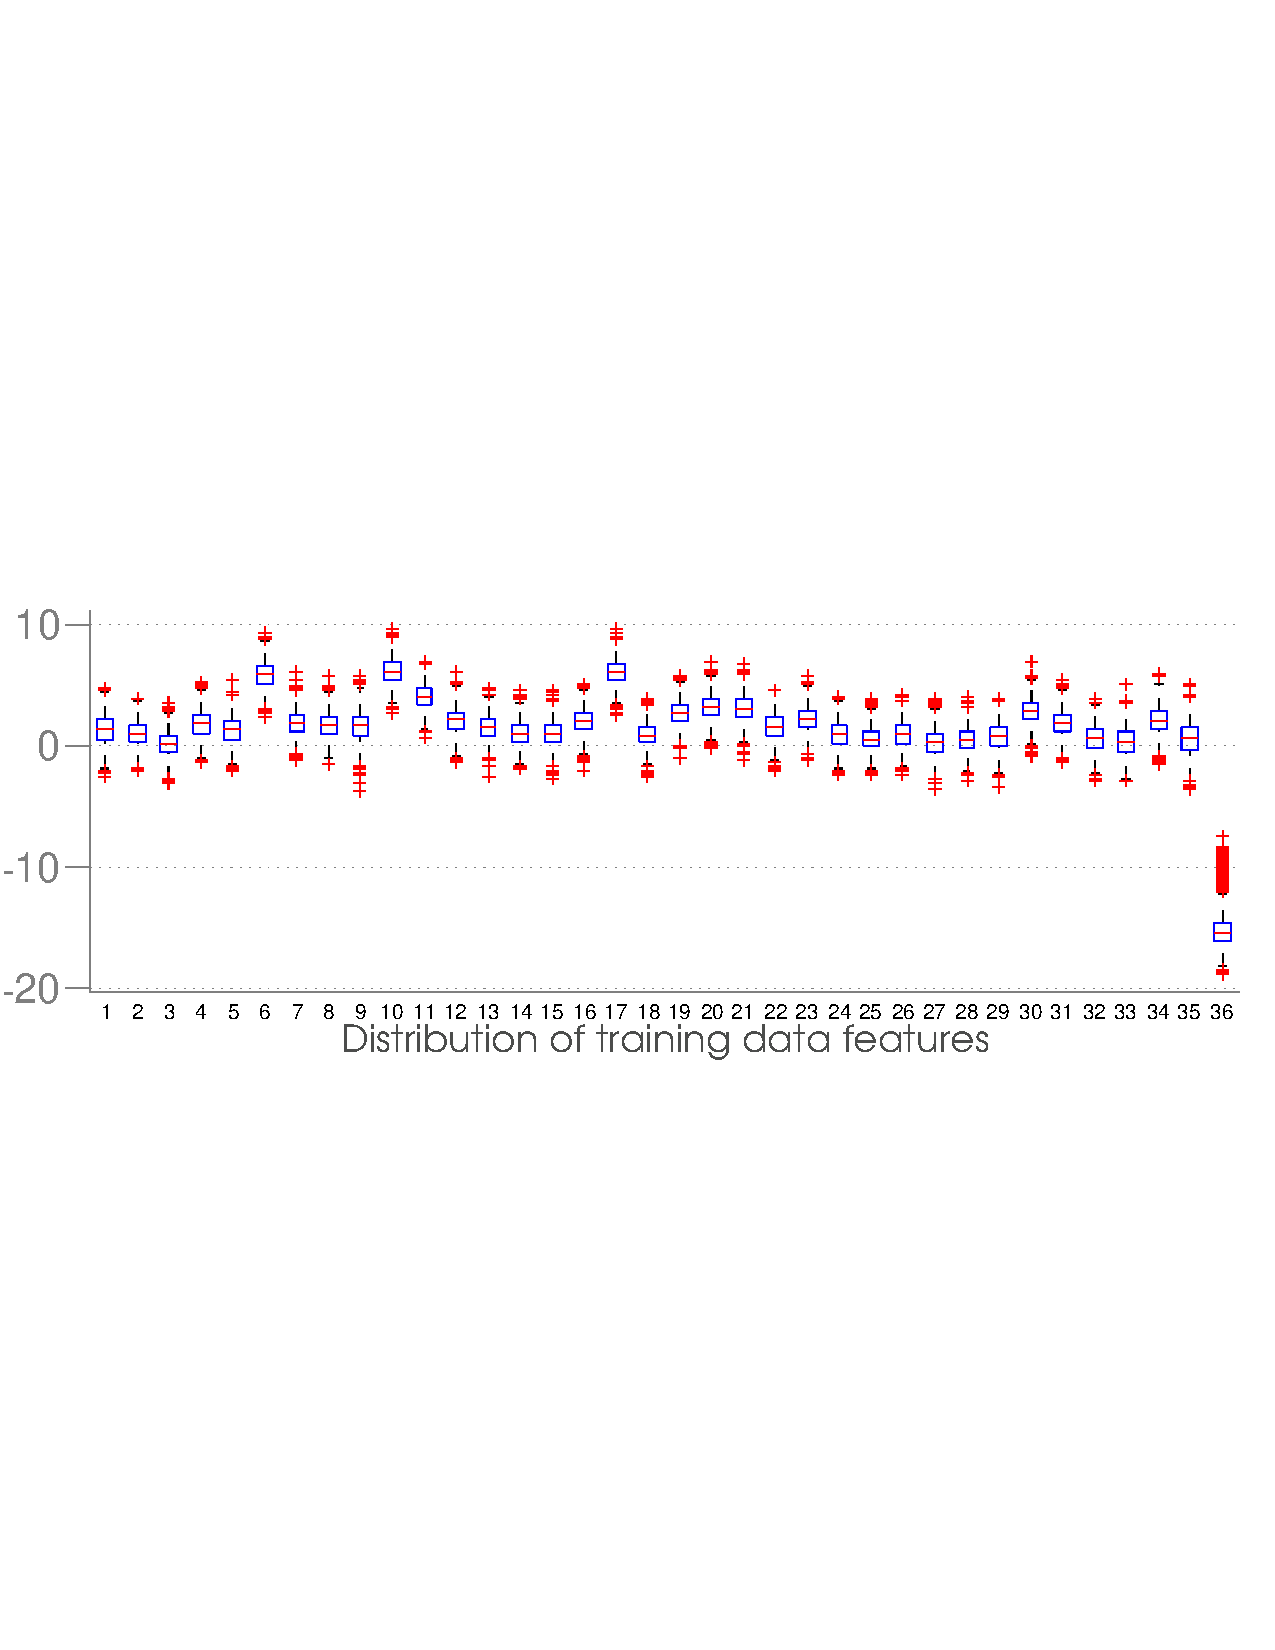
\includegraphics[width=\textwidth]{figures/distribution_regression_crop.pdf}
    \caption{Mean and standard deviation for the first 36 real valued variables of Xtrain. The input is not normalised and feature 36 is the only negative one.}
    \label{fig:dist_regression}
  \end{subfigure}
  \begin{subfigure}[b]{0.45\textwidth}
    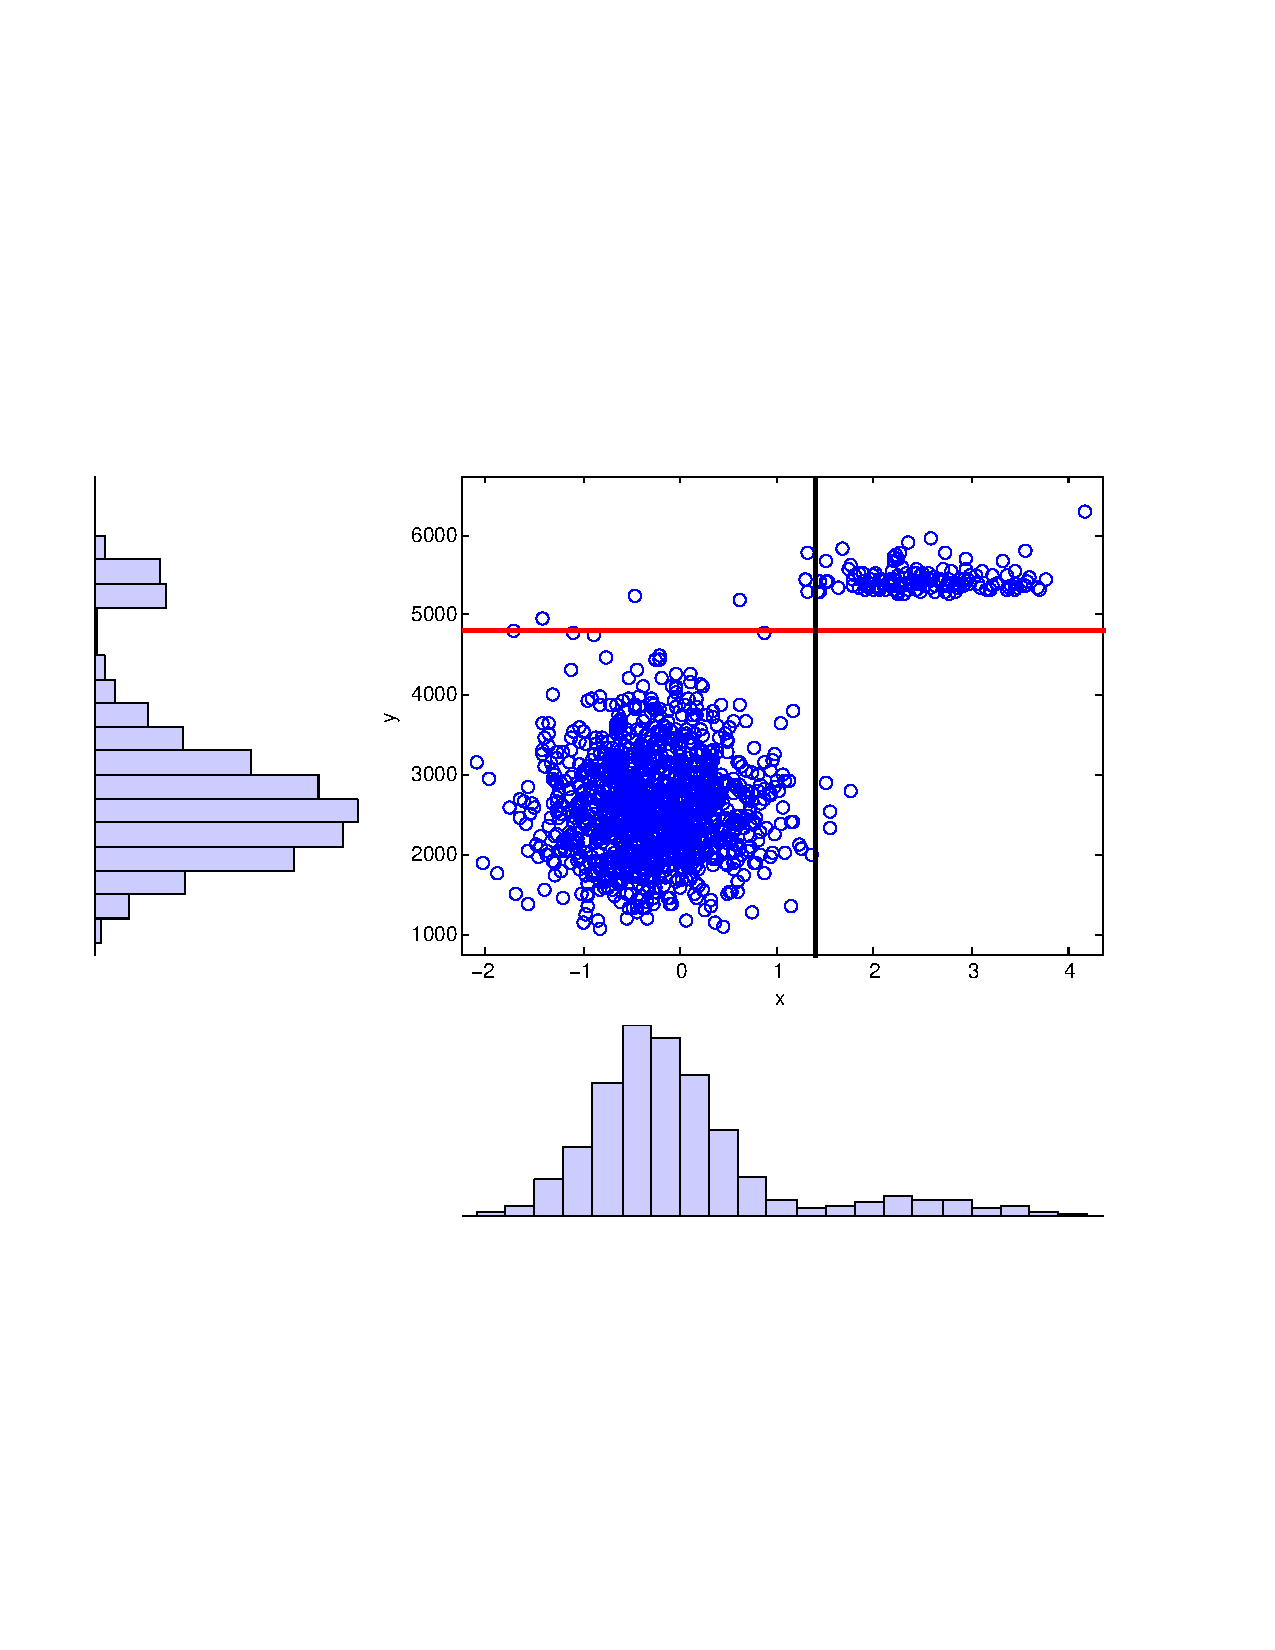
\includegraphics[width=\textwidth]{figures/feature36_crop.pdf}
    \caption{Feature 36 versus output values. X = 1.4 (black line) and y = 4900 (red line)  provide a good separation of the two blobs.}
    \label{fig:feature36}
  \end{subfigure}
  \caption{• Data visualization. }
\end{figure}

We visually observed some linear correlations between certain features such as feature 2 and 24, 13 and 16, 17 and 20, but we decided to keep them since we did not have time to experiment with their removal or to test their signifcance. This is corroborated by the fact that $Xtrain$ is rank deficient, it has 57 columns after the use of dummy variables but rank 50.

If the input is normally distributed with mean 0 and std 1, then
 $99.99\%$ of the samples appear between the values -3.891 and 3.891. We therefore remove any points that are outside this interval, considering them outliers.

\subsection{Ridge regression Baseline methods}
 

\subsection{Feature transformations}
We tried polynomial and exponential transformations of the features.
The exponential transformation did not prove to work well and we focused on polynomial regression.
We only transformed the first 35 variables and kept the categorical variables as they are since  polynomial transformation of categorical variables does not have an intuitive interpretation. 

The degree of the polynomial was varied from 1 to 10 for both blob-models. In $Fig$\ref{fig:degree_blob1},\ref{fig:degre_blob2} we plotted the mean training and validation $RMSE$ for the degree varying only between 2 - 10 and 2 - 6 respectively for readability (for the other values the RMSE was too big).

Using 5-fold cross validation with $\lambda = 1e-5, \alpha = 0.1$ we
notice that a polynomial of degree 3 is a good fit for the first model. Increasing it further leads to overfitting, since the training errors becomes very small and the validation error increases. For the second model, using  $\lambda = 0.001, \alpha = 0.1$ we obtain a best fit for a polynomial of degree 2.

\begin{figure}[h]
  \begin{subfigure}[b]{0.45\textwidth}
   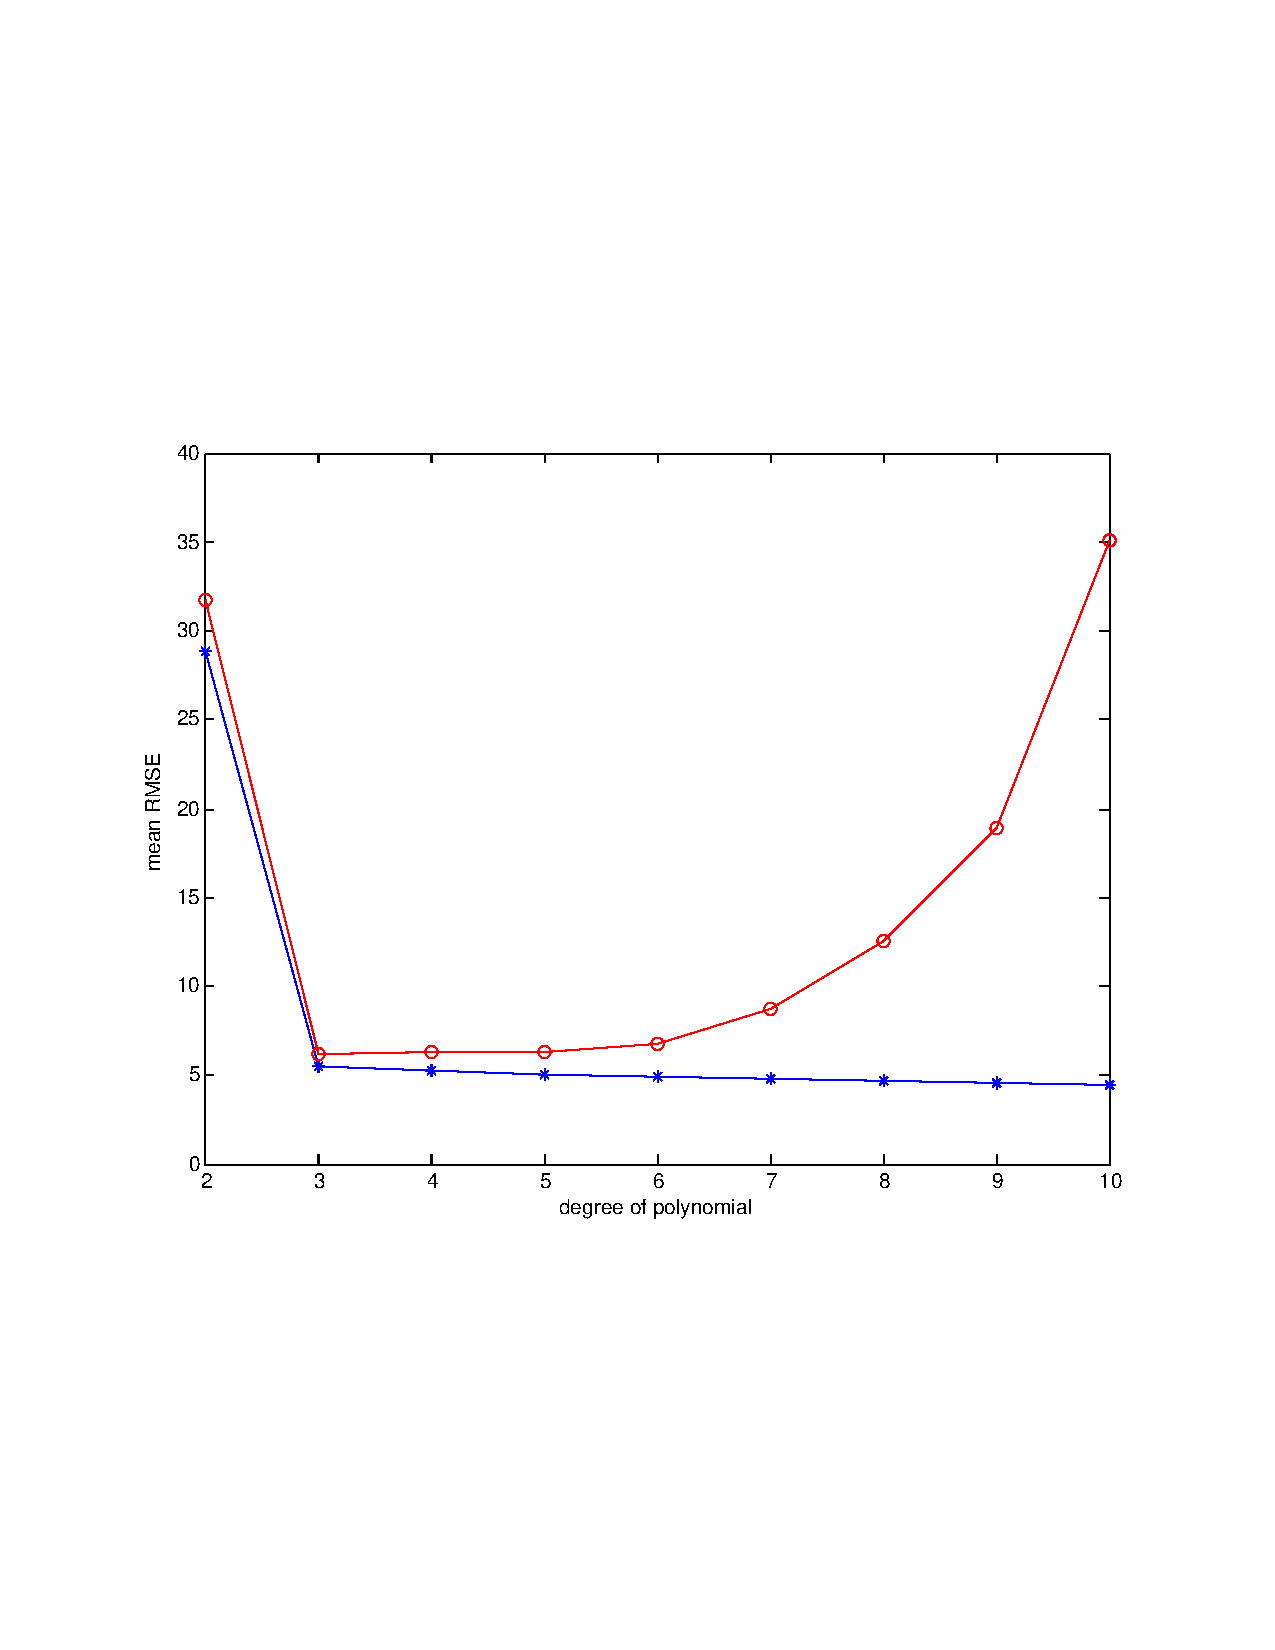
\includegraphics[width=\textwidth]{figures/degree_polynomial_blob1_crop.pdf}
    \caption{First Blob. Mean RMSE for training set \newline (blue curve) and testing (red curve) versus poly-\newline nomial degree. The errors were computed using\newline 5-fold cross-validation.}
    \label{fig:degree_blob1}
  \end{subfigure}
  \begin{subfigure}[b]{0.45\textwidth}
    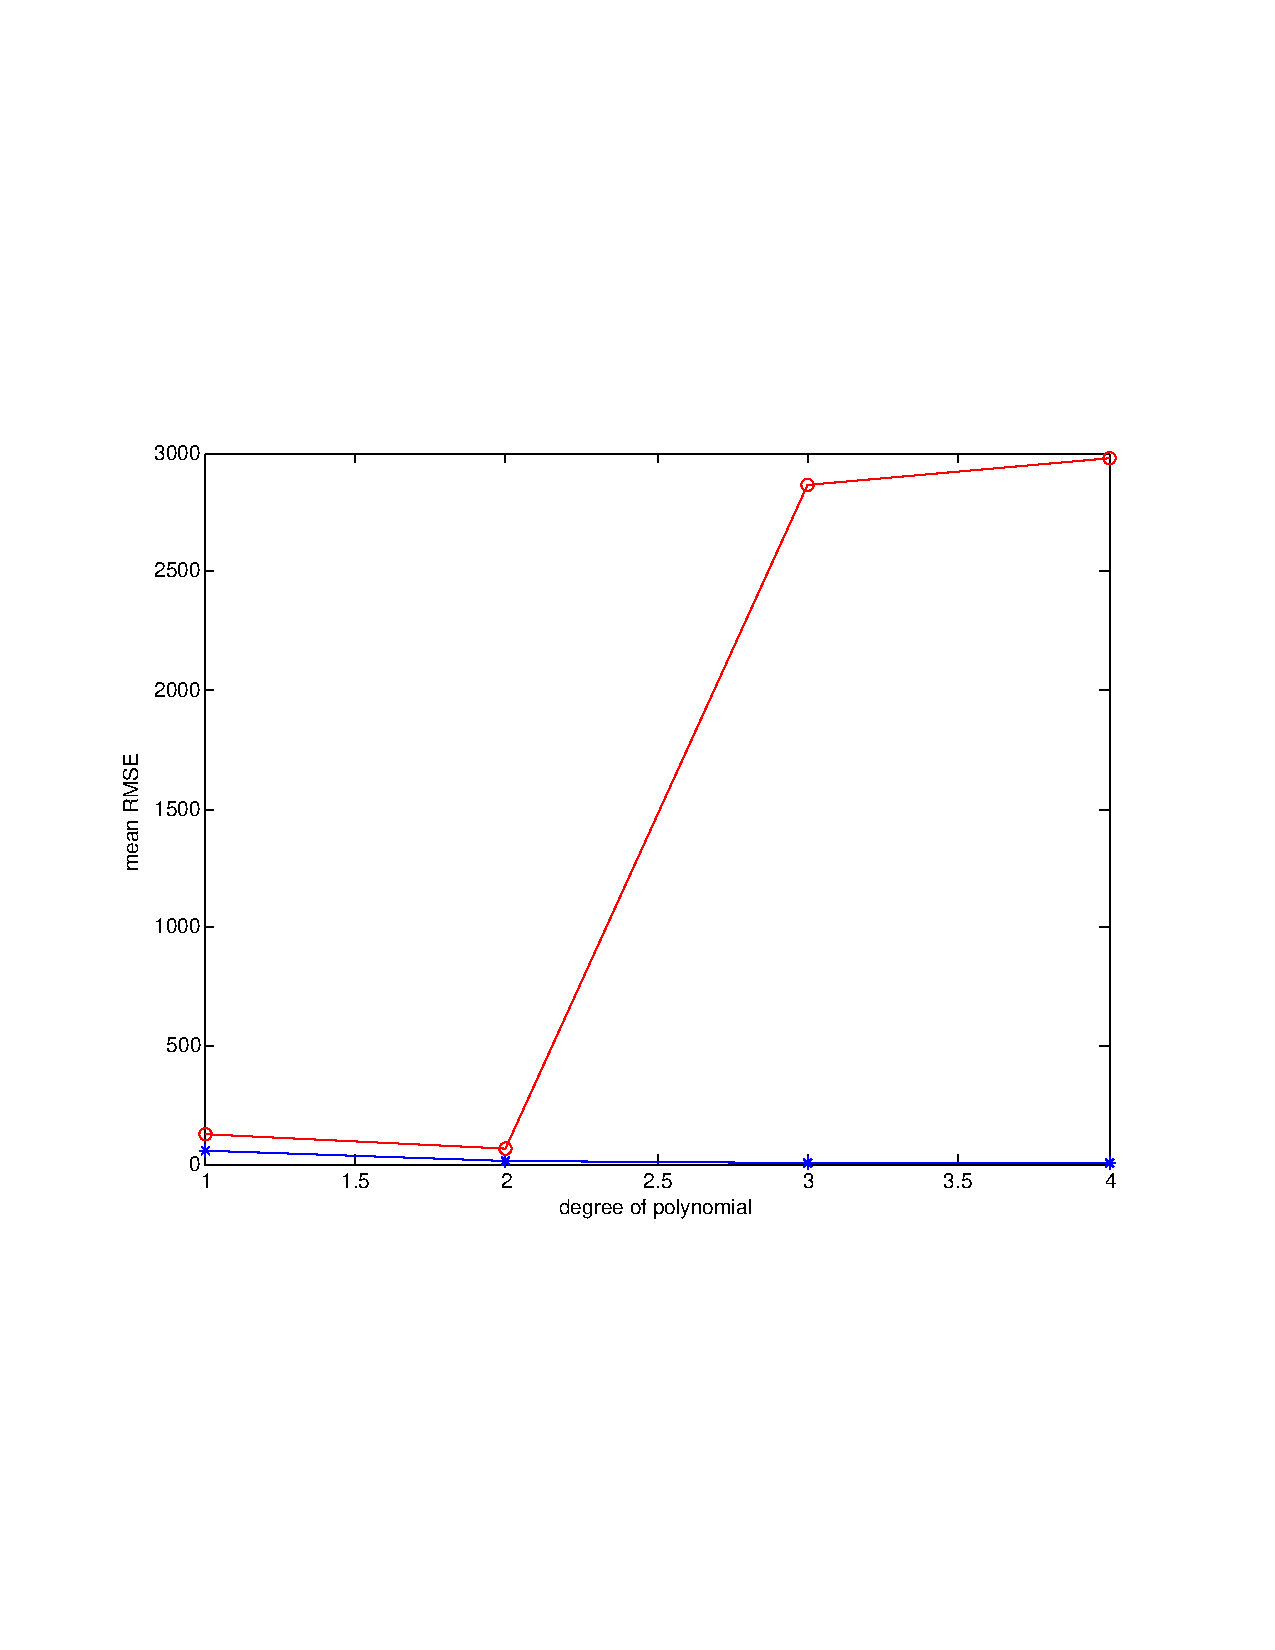
\includegraphics[width=\textwidth]{figures/degree_polynomial_blob2_crop.pdf}
    \caption{Second Blob. Mean RMSE for training set (blue curve) and testing (red curve) versus polynomial degree. The errors were computed using 5-fold cross-validation.}
    \label{fig:degre_blob2}
  \end{subfigure}
  \caption{• Selection of polynomial degree}
\end{figure}

We increased lambda to prevent overfitting, since we have 10 times less samples for the second model. However, we still noticed that our RMSE for the validation set  was  bigger for the second blob. This might be due to the fact that we have a very small set for both training and testing of the second model.

Both polynomial regression models significantly outperform the normal ridge regression, which gave a RMSE > 100.

Model1 mean  5.4649( std 0.0579) mean 6.2188( std 0.4801)
Model2 mean   11.7039( std 2.0178) mean  53.1940( std 14.5599)


Note also that our final RMSE (reported on the whole training data) is smaller that the sum of the two separated RMSE.
\TODO{write here about best RMSE for both models separate, and for the final one.}

\section{Classification}
\subsection{Data description}
We have a two-class classification problem. The training data $Xtrain$ contains 1500 observations, each 32 dimensional. One training sample has 31 real valued features and 1 categorical feature, the 14th feature. Our task is to predict the category for unseen test data, consisting in 1500 samples. We measure the accuracy of our estimation using $RMSE$, $0-1 loss$ and $log-loss$. 

\subsection{Data visualization and cleaning}
We noticed that the samples were not equally distributed among classes, about $35\%$ of the samples were coming from one class and $65\%$ from the other. We did not have time to study the implications of this on our model estimation. We changed the labeling from -1/1 to 0/1. 

The training data was again not centered as seen from $Fig.$\ref{fig:dist_classification}
We noticed more outliers in the data of classification than in the one from regression. After removing the outliers and changing feature 14 to a dummy variable we normalized the data to have 0 mean and std 1.
{%%#figures/distribution_classification.png}
\begin{figure}[h]
  \begin{subfigure}[b]{0.5\textwidth}
   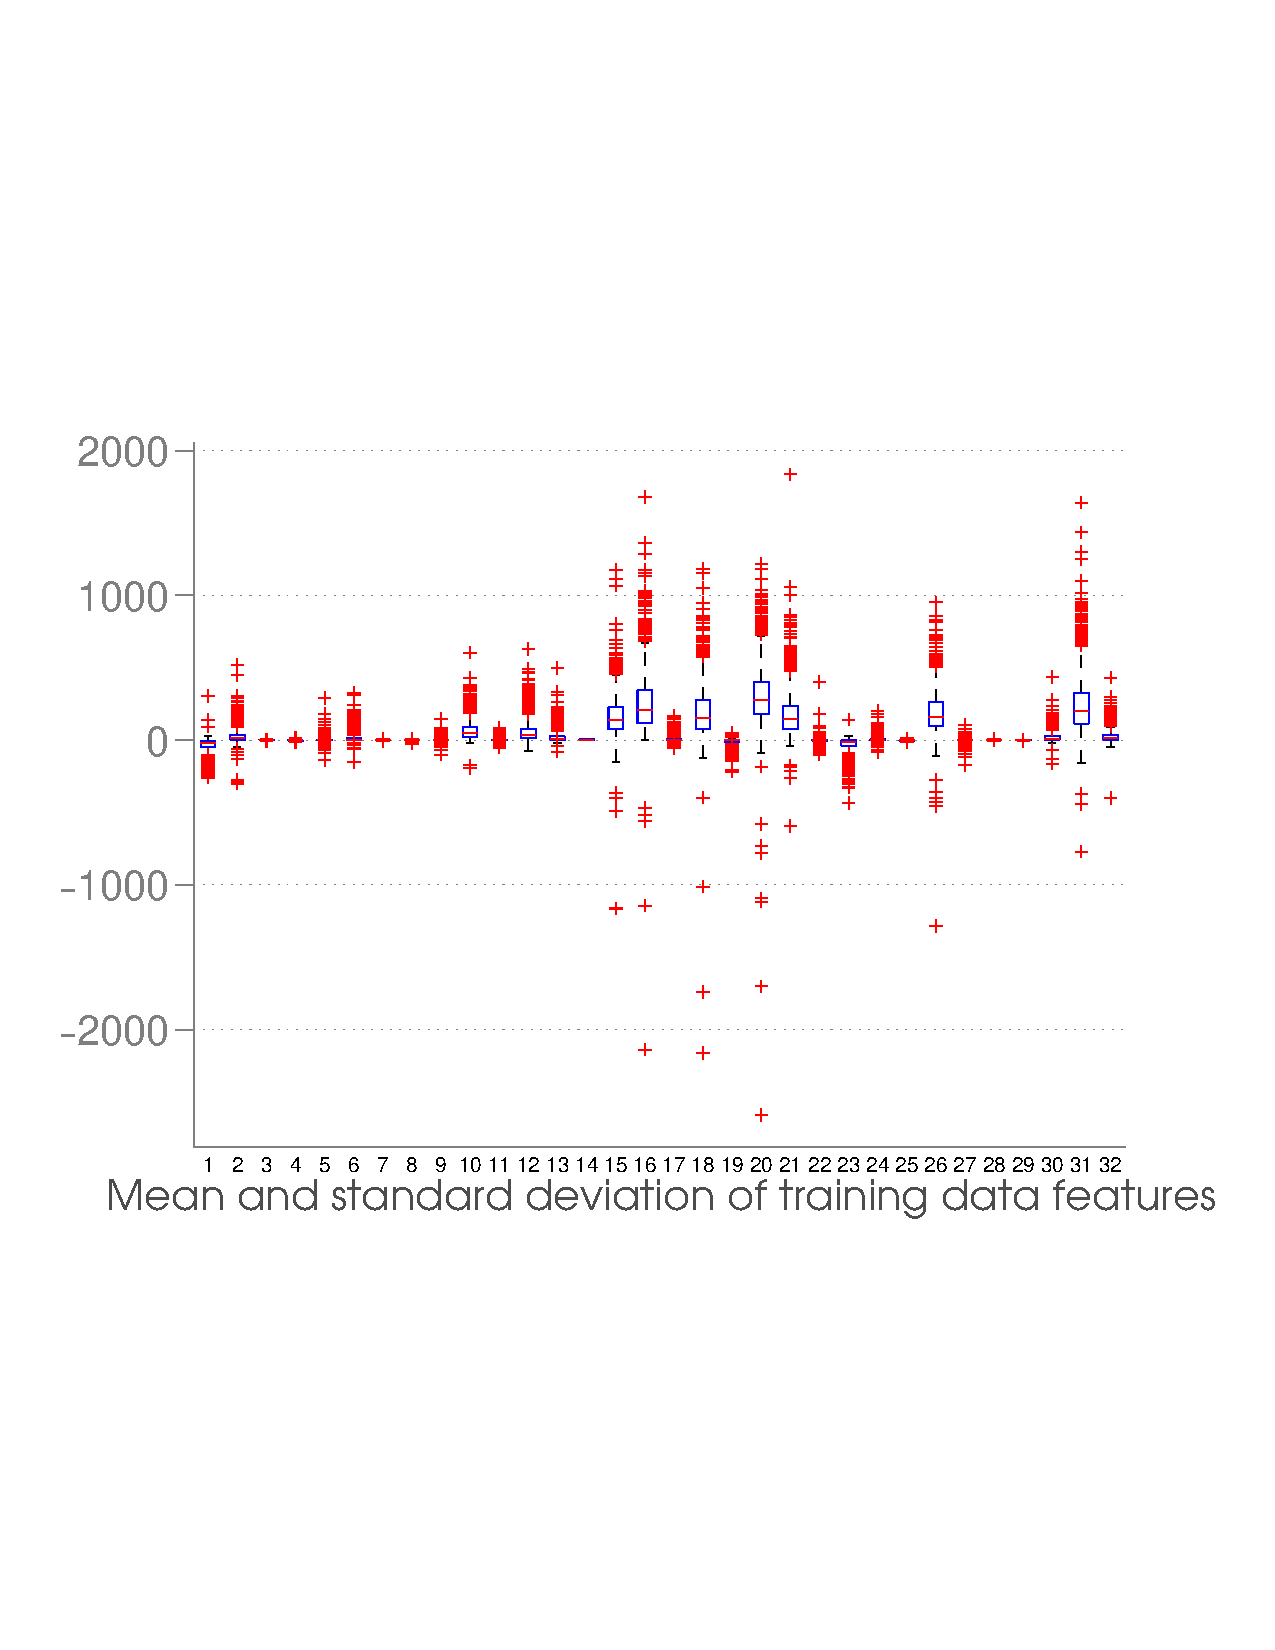
\includegraphics[width=\textwidth]{figures/classification_distribution.pdf}
    \caption{Mean and standard deviation for the training data features. The input is not normalised and contains outliers.}
    \label{fig:dist_classification}
  \end{subfigure}
  \caption{• Data visualization. }
\end{figure}

\subsection{Logistic regression}
\subsection{Feature transformation}

\section{Summary}


\subsubsection*{Acknowledgments}

\subsubsection*{References}

\end{document}
